\hfill \newline
\phantom{ } We built the circuit in figure \ref{fig:cir} with a resistor of $10\mathrm{k\Omega}$ and a capacitor of
$0.01\mathrm{\mu F}$. We set the function generator to provide a square wave input with the period $T=4.00000000\mathrm{ms}$ and the voltage of $V_{pp}=5\mathrm{V}$ with offset $+2.5\mathrm{V}$, which generates a square wave of maximum voltage $5\mathrm{V}$ and minimum $0\mathrm{V}$.

\begin{figure}[!htbp]
	\centering
	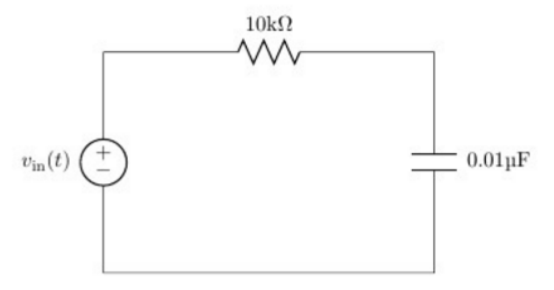
\includegraphics[width=\linewidth]{images/circuit.PNG}
	\caption{RC circuit for square wave input analysis}
	\label{fig:cir}
\end{figure}

We used channel 1 of the oscilloscope to verify the input and measured the output voltage of the capacitor by channel 2. Figure \ref{fig:osc1} is the screen output of two and half cycles.

\begin{figure}[!htbp]
	\centering
	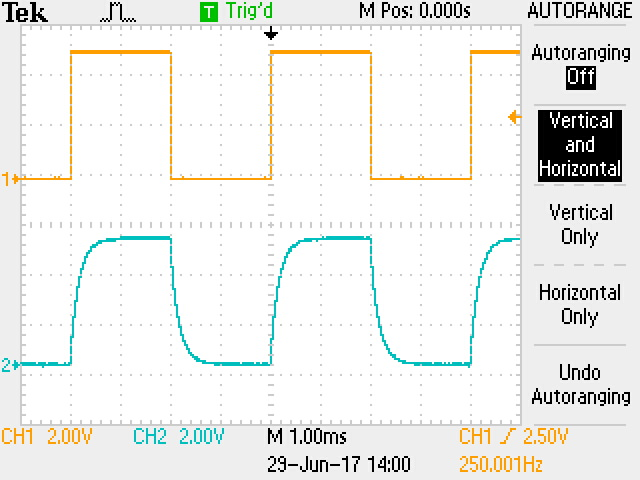
\includegraphics[width=0.95\linewidth]{images/osc1.JPG}
	\caption{The waveform of input and measure}
	\label{fig:osc1}
\end{figure}

\textbf{Analyze \#1:} \newline
\phantom{ } The oscilloscope did display the same waveform plotted in Prelab\#7. They are of the same shape, and both of their peaks and valleys reach the input waveform. Meanwhile, no obvious difference is found. \newline

Using the \textit{Cursor} menu, we recorded the period $T$, as well as the range of the output signal. Then we measured the time value of the $10\%$, $90\%$, and $50\%$ point of $V_{out}$. The results are shown in table \ref{tab:mea}.

\begin{table}[!htbp]
	\centering
	\caption{Measurements of the output signal}
	\begin{tabular}{lcl}
		\toprule
		name & value & \\
		\midrule
		period & $4.000\mathrm{ms}$ & \\
		max voltage & $5.120\mathrm{V}$ & \\
		min voltage & $0.000\mathrm{V}$ & \\
		time of $10\% V_{out}$ (LH) & $16.0\mathrm{\mu s}$ & \\
		time of $90\% V_{out}$ (LH) & $364\mathrm{\mu s}$ & \\
		time of $50\% V_{out}$ (LH) & $116\mathrm{\mu s}$ & \\
		time of $10\% V_{out}$ (HL) & $??\mathrm{\mu s}$ & \\
		time of $90\% V_{out}$ (HL) & $??\mathrm{\mu s}$ & \\
		time of $50\% V_{out}$ (HL) & $??\mathrm{\mu s}$ & \\
		\bottomrule
	\end{tabular}
	\label{tab:mea}
\end{table}

\textbf{Analysis \#2:} \newline
\phantom{ } After calculating the rise time, fall time, and delay time of the RC circuit, we got table \ref{tab:cal}

\begin{table}[!htbp]
	\centering
	\caption{Measurements of the output signal}
	\begin{tabular}{lcccl}
		\toprule
		name & actual value & theoretical value & PE & \\
		\midrule
		rise time & $348\mathrm{\mu s}$ & ${220\mu s}$ & $58.2\%$ & \\
		fall time & $??\mathrm{\mu s}$ &  ${220\mu s}$ & $??\%$ & \\
		delay time (LH) & $116\mathrm{\mu s}$ & ${69\mu s}$ & $68.1\%$ & \\
		delay time (HL) & $??\mathrm{\mu s}$ &  ${69\mu s}$ & $??\%$ & \\
		\bottomrule
	\end{tabular}
	\label{tab:cal}
\end{table}

